%% LyX 2.0.5.1 created this file.  For more info, see http://www.lyx.org/.
%% Do not edit unless you really know what you are doing.
\documentclass[english]{article}
\usepackage[T1]{fontenc}
\usepackage[latin9]{inputenc}
\usepackage{graphicx}

\makeatletter

%%%%%%%%%%%%%%%%%%%%%%%%%%%%%% LyX specific LaTeX commands.
\newcommand{\noun}[1]{\textsc{#1}}

\makeatother

\usepackage{babel}
\begin{document}

\title{STNUM - TP1\\
LOGICIEL R ET RAPPEL DES PROBABILIT�S}


\author{\noun{Juste Raimbault}}

\maketitle

\section*{Question 1}

The command {rnorm} generates random numbers following a centered
gaussian law, for which the density is, if $\sigma$ is the standard
deviation, $f(x)=\frac{1}{\sqrt{2\pi\sigma^{2}}}\cdot e^{-\frac{1}{2}\cdot\frac{x^{2}}{\sigma^{2}}}$.
The maximal value taken is then $\frac{1}{\sigma\sqrt{2\pi}}$, and
therefore we fix the upper bound for $y$ just a little above this
value (1.2 times, taking the maximum with the frequencies of the histogram,
since the bars can go above the theoretical curve), after having calculated
$\sigma$ by $\sigma=\{sd(x)\}$.


\section*{Question 2}


\section*{Question 3}

\begin{figure}


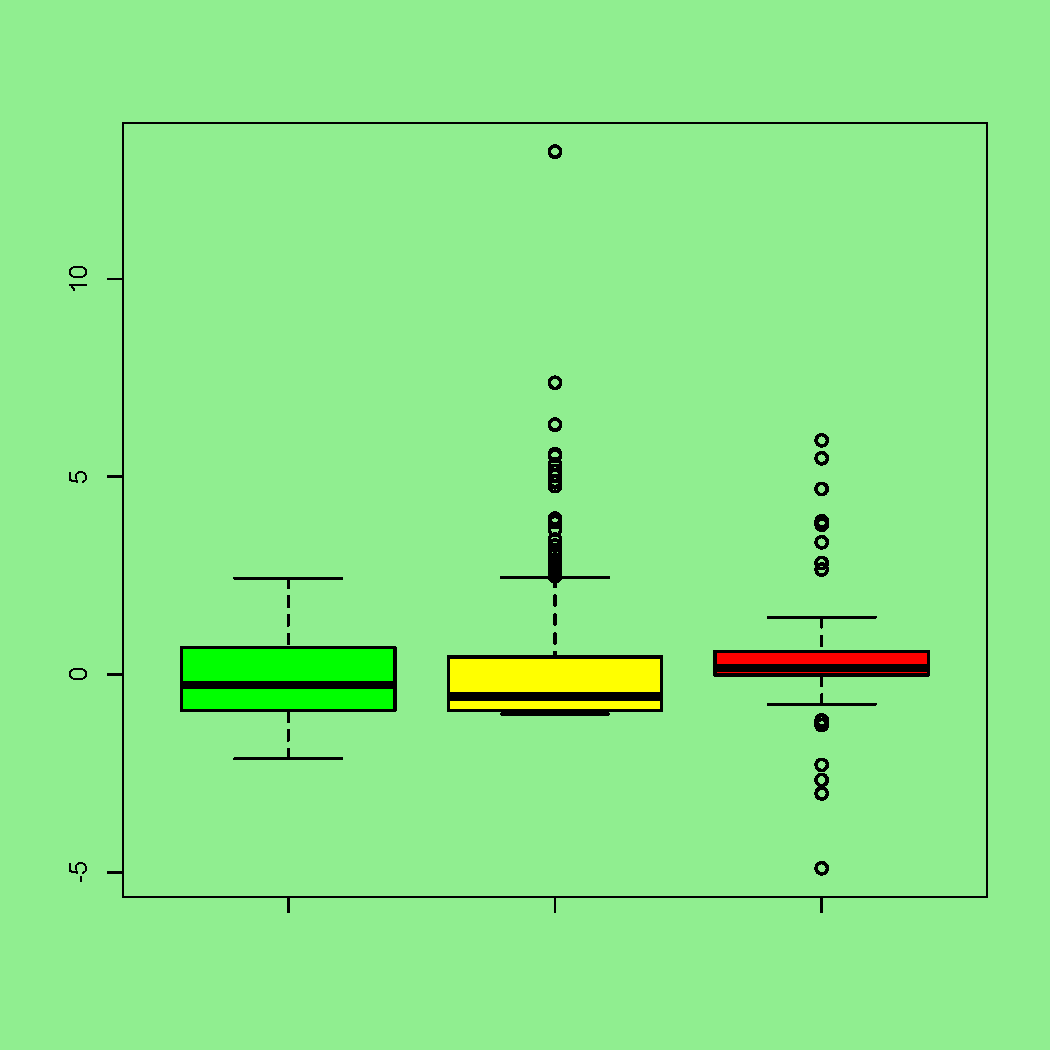
\includegraphics[scale=0.7]{boxplot35}\caption{Boxplots of 3.5}


\end{figure}

\end{document}
